%% This is the Chapter 4

%\begin{hyphenrules}{nohyphenation}
\chapter{MODELLING TRAIT-DEPENDENT RATES OF TRAIT EVOLUTION USING CONTINUOUS MATHEMATICAL FUNCTIONS}
%\end{hyphenrules}

\section{Abstract}

To be done.

\section{Introduction}

There is a striking contrast in the degree of phenotypic diversity between clades across the tree of life. A trivial component of such discrepancy is time, because older clades are expected to have accumulated higher diversity both in number of species and phenotypic divergence than younger groups. However, such simple relationship does not hold for many groups, since several factors can generate divergent macroevolutionary patterns. For instance, adaptive radiations can drive rapid differentiation of lineages and, thus, cause increased phenotypic diversity on young clades. On the other end of the spectrum, evolutionary constraints to trait evolution can cause reduced phenotypic differentiation of lineages through time. The genetic architecture, function and fitness landscape associated with a trait can result in bounds that keep traits inside their adaptive zones over long time scales. These processes, however, are not exclusive. Transitions between adaptive zones are associated with rapid phenotypic changes as lineages move through the morphospace from a adaptive peak to another.

Adaptive radiations and the track of adaptive peaks by lineages are often associated with discrete events that change the tempo and mode of evolution of the group. The evolution of a novel trait, referred as key innovation, or the dispersal to a novel habitat are commonly attributed as explanations to bursts of diversification or changes in the direction of phenotypic evolution of a clade. However it is plausible that such changes are not due to discrete events on the macroevolutionary history of a group, since gradual changes in the pace of evolution can also result in increased differentiation among clades. Moreover, given that most studies are focused on the impact of discrete events on the tempo and mode of evolution, it is possible that gradual changes have been not detected in many groups.

% The main idea here is that the processes hypothesized to be responsible for rapid or slow rates of phenotypic evolution though time are often associated with discrete, sometimes rare, events in the history of clades. However, changes in the pace and mode of evolution have been shown to change gradually in the history of clades. Thus, there is a chance that such empirical patterns might not be well explained by hypothesis which focus changes to discrete regimes in the tree. In such cases we want to relate the increase or decrease of evolutionary rates in a continuous manner rates than dividing a phylogenetic tree into discrete regimes.
% I think that the best part of the argument have to do with the fact that we try to study radiations and changes in niche, or species diversification by relating it to discrete changes. But there are good reasons to think that changes in the pattern of macroevolution of lineages are associated with continuous changes in other factors. This is the main hook of this paper. I think that the use of novel models, such as BAMM, is a nice argument for the focus on continuous patterns more than discrete changes only.

Although adaptive zones are most often associated with external factors, such as environment and species interactions, the evolutionary correlation among traits can also be an important driver of phenotypic diversification. When traits are correlated due to special function, one trait can be bounded to a limited region of the morphospace due to the restrictions pose by selection on the performance of the set of traits.

% Best way to keep going on this introduction is to found very nice examples in which the evolution of a trait is related to another continuous variable. I can see body size, range size, or even behavioral characteristics as good candidates. Although temperature and latitude seems to be one of the largest drivers of evolution across the globe, I am not 100% sure if the idea of having environmental characteristics evolving on the tree is a good way to go.  

\section{Methods}

\subsection{Description of the model}
% The root for the Q matrix estimate using fitDiscrete might be different than when making stochastic maps with make.simmap. By default make.simmap will set the prior for the root as flat. I do not know what is the default behavior for fitDiscrete, however this is an important thing to be aware of. If the root behviour is very distinct, it might be a good idea to change something for them to be more compatible. One thing is that we have information about the root of the model since the BM model will have root close to the mean of the data.

Here we use continuous mathematical functions to model the rates of evolution of a trait (i.e., the response trait) under a Brownian-motion model (BM) with respect to the values of another trait (i.e., the predictor trait). The model aims to study the association between the macro-evolutionary patterns of a trait evolving on a phylogenetic tree and the rates of evolution of a second trait on the same tree. Figure \ref{fig:model_example} shows the fundamental concepts of the model. % A summary figure to explain the concept of the model. Try to use colors to associate the simmap on the branches of the tree and the function.
Both the predictor and response traits are continuous traits for the same set of species. The mathematical function represented by the line on Figure \ref{fig:model_example} describes the variation of evolutionary rates for the response trait in function of the trait values of the predictor trait. The difference between the present model and other phylogenetic comparative models of trait evolution with varying rates, such as AUTEUR, bayOU, and BAMM traits, is that these methods only fit rates of evolution for a single trait, informed by the distribution of trait values across the species, and the branch lengths and topology of the phylogenetic tree. In contrast, here we introduce the use of a second trait to inform the variation of rates of evolution across the branches of the tree.

The model can be sub-divided into two components; ancestral values for the predictor trait are mapped to the branches of the phylogenetic tree and evolutionary rate regimes for the response trait are assigned to the phylogeny in function of the map of ancestral predictor trait values. For this we first assign the predictor trait values to $\mathit{k}$ ordered categories defined by $\mathit{k}$ - 1 equidistant breakpoints across the range of the predictor trait values (see x-axis of Figure \ref{fig:model_example}). Then we estimate the evolutionary rate transitions among the $\mathit{k}$ categories with a model that restricts transition rates to happen only between neighbouring states. For example, a transition from the trait value category $\mathit{k_{i}}$ to a larger trait value category $\mathit{k_{i+3}}$ need to be preceded by transitions to and from the intermediary categories $\mathit{k_{i+1}}$ and $\mathit{k_{i+2}}$. The number of categories reflects how fine-grained is the model with respect to the macro-evolutionary patterns of the (continuously distributed) predictor trait; larger $\mathit{k}$ produce a more fine detailed model whereas smaller $\mathit{k}$ yield a more coarse model.
% The comment made in this paragraph calls for a sensitivity test regarding the number of categories used to describe the predictor trait. This is an essential result and should be included in the chapter.

The transition rates between the $\mathit{k}$ categories of the predictor trait can be estimated using a meristic Markov model (Mkn). Here the predictor trait is assumed to evolve under a single homogeneous rate or multiple rate regimes. Homogeneous rate can be described by constraining all transition rates to be equal whereas more complex evolutionary patterns can be described by allowing transition rates to and from each category to vary. Of course, one compare and choose the model that best describes the evolutionary history of the predictor trait across the branches of the phylogenetic tree. As the number of categories ($\mathit{k}$) increases the single rate Mkn model becomes equivalent to a single rate Brownian-motion (BM) model whereas the unconstrained Mkn model spans heterogeneous rate trait evolution models such as multiple rate BM, BM with a trend and Ornstein–Uhlenbeck (OU). However, the Mkn model fits a single transition matrix to the phylogenetic tree and, as a result, can only be equivalent to time-dependent models, such as the accelerated/decelerated (ACDC) and early burst (EB), if the predictor map shows a time-dependent structure.
% Although the free model spans the 'BM with a trend', because of the way the estimation works and because the categories are defined using the tip data, it is very unlikely (maybe impossible) for the 'BM with a trend' model to be one of the estimated models.

In order to map ancestral values of the predictor trait to the branches of the phylogenetic tree we generate multiple stochastic histories for the trait categories using the estimated Mkn transition matrix. Each of these maps associate the branches of the phylogeny with a category for the ancestral values of the predictor trait. Then we use a mathematical function to map these predictor trait regimes to evolutionary rate regimes for the response trait and compute the likelihood of a multiple rates Brownian-motion model with the response trait as the tip data.

\subsection{Mathematical functions and model choice}
% Talk a little that we are using MLE estimation, but that MCMC or even RJMCMC can be implemented. This is more suitable to the Discussion section.

Virtually any mathematical function can be used to map values of the predictor trait categories to evolutionary rate regimes of the response trait. Different functions can be fit to the data using maximum likelihood (ML) and compared using standard model choice approaches such as Likelihood-ratio tests (LRT) for nested or the Akaike information criterion (AIC) for non-nested models. Using model choice criteria that penalizes for the number of parameters (such as AIC) is desirable, since distinct functions of varying complexity can produce identical maps. Some mathematical functions are commonly applied across a series of biological disciplines and are likely to be erected as \textit{a priori} hypotheses for the macro-evolutionary association between a plethora of traits. Figure \ref{fig:bio_functions} shows a collection of functions that describe patterns commonly observed in biological data, especially in studies of trait evolution using phylogenetic trees.

One of the advantages of our approach is that the number of parameters varies with respect to the chosen mathematical function rather than the number of categories used to describe the predictor trait (see Figure \ref{bio_functions}). This is a result of maximizing the likelihood of the data with respect to the parameters of the mathematical function rather than to the rate regimes directly. Thus, we can use a large number of rate regimes in order to model a trait with  (semi-)continuously varying rates of evolution across the phylogeny without increasing the number of parameters of the model. This aspect of the model is similar to the strategy implemented in BAMM traits, which uses an exponential function to describe the continuous decrease or increase of rates of trait evolution through time. % DOUBLE CHECK IF BAMM WORKS LIKE THIS!!

\subsection{Model implementation}

We implemented the model as a R package named \texttt{`phylofx'}. The package offers a simple interface to fit continuous mathematical functions to model the variation of evolutionary rates of a response trait in function of a predictor trait across the branches of a phylogenetic tree. All mathematical functions showed on Figure \ref{fig:bio_functions} are available in the package and can be chosen from a simple menu. The package also have options for users to define their own mathematical functions.

\subsection{Performance simulations}
% One aspect of the model that was not explored by the simulations is the possible case in which rates of evolution are heterogenic over the phylogeny but that the shifts have no relation with any other trait. What happen with the model selection? It is likely that a more complex model will be selected in this case. Maybe it is a good idea to use another model when doing this tests. Maybe we can test the AIC scores against a aeuteur model? The aeuteur model will accomodate heterogenic rates of trait evolution without relating it to any other trait. This is a good thing to think about and is similar to the issue addressed by Beaulieu and O'Meara.

To check the performance of the method we will focus in three very common, but distinct, nested models: a constant relationship, with homogeneous evolutionary rates ($\sigma^{2}$=0.5); a step function, with two distinct rates separated by an instantaneous transition step ($\sigma^{2}_{left}$=1, $\sigma^{2}_{right}$=0.5, break point=mean of predictor trait); and a linear function, with a continuous relationship between the predictor and the response traits. For the linear function we defined $\beta_{1}$=0.5, set of predictor trait values at the tip as $X$, and defined the intercept such that:

\begin{equation}
\beta_{0} = \beta_{1} \ min X - 0.1
\end{equation}

We generated a phylogenetic tree with 200 species using a pure-birth model (tree height=1). Then we simulated a predictor trait following a single rate BM model ($\sigma^{2}$=0.5) and divided it into 10 trait categories mapped to the branches of the tree. We will refer to the result of this simulation as the true mapped tree. We used the true mapped tree to assign evolutionary rate regimes to the branches following one of the mathematical functions described above and simulated the response trait under a multi-rate BM model. We repeated this process in order to produce 100 datasets for each mathematical function.

In order to fit the models to the generated data, we estimated a meristic Mkn transition matrix for the predictor trait with $\mathit{k}$=5 and equal transition rates. We produced 10 stochastic mapping histories based on this transition matrix and performed a maximum likelihood estimate for each of the mathematical functions under each of the stochastic mapping histories. We chose the best model by comparing the mean pairwise AIC values across all stochastic maps. We repeated model fit and model test for each of the 300 simulated datasets. We computed error rates as the frequency in which the model used to generate the data was not selected as the best model.

Preliminary tests showed that it is often difficult to find the global maximum likelihood for the parameters of the model using minimization algorithms. Thus, we applied three distinct strategies to generate the starting point for the searches. First we generated starting points by drawing from a flat distribution with large range of parameter values (from -400 to 400). Starting points generated using this approach are unlikely to be close to the global maximum but provide an acceptable representation of the parameter space. We refer for the approach as `wide'. Second we used a more informed approach by optimizing the parameters of the mathematical functions to produce evolutionary rates equal to $\sigma^{2}$ estimated for a homogeneous BM model with the response trait as the tip data for the tree. Then we defined a narrow range of parameter values (-10 and +10 units) around the best fit and used this distribution to draw starting points. We refer to this strategy as `narrow'. Finally, we applied the most informative strategy by setting the starting point of the ML searches as the true parameter value for the models. When performing analysis with a model that did not generated the data we set the mathematical function as to minimize the distance relative to the evolutionary rates predicted by the true model. We defined this search strategy as `fixed'. We compare and discuss results among the different search strategies.

\subsection{Sensitivity to trait categorization}
% In a subsequent test I might be able to make a more comprehensible thing by increasing the number of categories of the true model or even making a full continuous simulation.

Our model associates the evolutionary rates of a continuous response trait to the trait values of a continuous predictor trait by transforming the data into ordered categories. On one hand, if the number of trait categories is large enough the trait evolution model converges with continuous models, such as Brownian-motion. On the other hand, this raises concerns about the adequacy of the model and parameter estimates when one applies only a small number of trait categories.

In order to test the sensitivity of the model to the number of trait categories ($\mathit{k}$), we simulated data following the same approach described above for performance simulations. However, we increased the number of trait categories to 15 and simulated datasets only with the linear function. We estimated parameter values for the linear model and performed model test using $\mathit{k}$ equal to 15, 10, and 5. Then we computed the distance between estimated parameter values to the true parameter values and the frequency that the generating model was chosen as the best model.

\section{Results}

First we computed the proportion in which each of the generating models was recovered by model selection using the Akaike information criterion (AIC), including the uncertainty associated with the use of stochastic mapped histories and the different approaches used to define the starting point for the maximum likelihood searches. Table \ref{tab:best_aic_sims} shows the number of times that each model had the best AIC score across all 100 simulated datasets. Almost all replicates, independent of search strategy, recovered the true model when data was generated using a constant evolutionary rate throughout the tree. Table \ref{tab:support_true_model} also shows that there are strong support for the constant model when compared to the other models. In contrast, results from the linear and step models show that the strategy used to choose the starting point for the optimizer has important influence on AIC scores.

For the linear model, in which rates of evolution are positively correlated with the predictor trait, both the `wide' and `narrow' starting point distributions (Table \ref{tab:best_aic_sims}) show a very strong skew towards the step model being the best model in the set of alternative models. The pattern drastically change when the initial point for the optimizer is set to be equal to the parameter values that generated the data (i.e., `fixed' strategy). The majority of the replicates recover the generating model as the model with highest AIC scores, although the step model is still found to have the best AIC score in 22 out of 100 simulations. When we compute the number of replicates that showed mean pairwise $\Delta$AIC scores across stochastic mapped histories larger than 2 AIC units, we can see that evidence in favor of the linear model was only found among the majority of simulation replicates using the `fixed' search strategy (Tables \ref{tab:support_true_model} and \ref{tab:reject_true_model}). When any other starting point scheme is employed, the performance of the linear model is low and alternative models often show better support.

Data generated under the step model show the reverse pattern when compared with the linear model. The most wide starting point schemes `wide' and `narrow' returned the generating model as the model with best AIC scores for the majority of replicates (Table \ref{tab:best_aic_sims}). The difference among AIC scores is also strong and in favor of the step model (Tables \ref{tab:support_true_model} and \ref{tab:reject_true_model}). On the other hand, the most informative starting point scheme (`fixed') results in every model showing the best AIC score with similar frequency among the simulation replicates (Table \ref{tab:best_aic_sims}). When computing pairwise mean $\Delta$AIC differences among models, there are more support in favor of the step model (Table \ref{tab:support_true_model}) than any other model (Table \ref{tab:reject_true_model}).

Model choice with the Akaike information criterion (AIC) uses the likelihood and the number of parameters to compare models, however it is also important to evaluate the parameter estimates for each model. For this we plotted the distance between the estimates of evolutionary rate and the true values of the rate for each of the five predictor trait value categories (Figures \ref{fig:chart_const}, \ref{fig:chart_linear} and \ref{fig:chart_step}). When data was simulated with the constant model, parameter estimates under the generating model are much closer to the true rates and the variance is much smaller than estimates using alternative models (Figure ). The step function show a good overall fit, with distances centred on zero and reasonable variance. In contrast, the linear model shows the worse fit, since rates of evolution are often estimated to be orders of magnitude larger than the true parameter value.



Figure \ref{fig:chart_const} are results with data generated under constant rate, Figure \ref{fig:chart_linear} are results with the linear function as the true model and Figure \ref{fig:chart_step} with the step function as the true model. For data generated using the constant model, 

% A similar, but also from a very different approach, is to ask about how good is these models to explaing the observed data? We can do this with parametric bootstraps. I can make plots comparing the distance from the observed data and the simulations for each of the estimated models.

\pagebreak

\begin{table}[h]
\caption[Number of times each model showed the best Akaike information criterion (AIC) score across 100 simulations using different search strategies.]{Number of times each model showed the best Akaike information criterion (AIC) score across 100 simulations using different search strategies. For each simulation AIC was computed as the mean AIC score across stochastic mapped histories. `Wide' denotes searches in which starting points were randomly draw from a wide uniform distribution of parameter values. `Narrow' and `Fixed' use more informed starting points for the MLE searches: the first draw from an uniform distribution around the parameter values after setting the function to produce rates of evolution equal to the rate estimated using a single rate Brownian motion model; the second sets the starting point as close as possible to the rates that generated the data.}
\label{tab:best_aic_sims}
\begin{center}
\begin{tabular}{ccccc}
\hline 
\textbf{True model} & \textbf{Search strategy} & \textbf{Constant} & \textbf{Linear} & \textbf{Step} \\ 
\hline 
\noalign{\vskip 2mm} 
Constant  & Wide & 86 & 0 & 14 \\
Constant  & Narrow & 88 & 0 & 12 \\
Constant  & Fixed & 90 & 0 & 10 \\
\noalign{\vskip 2mm} 
Linear  & Wide & 6 & 2 & 92 \\
Linear  & Narrow & 7 & 0 & 93 \\
Linear  & Fixed & 7 & 71 & 22 \\
\noalign{\vskip 2mm} 
Step  & Wide & 30 & 1 & 69 \\
Step  & Narrow & 27 & 0 & 73 \\
Step  & Fixed & 28 & 28 & 44 \\
\noalign{\vskip 2mm} 
\hline
\end{tabular}
\end{center}
\end{table}

\begin{table}[h]
\caption[Number of times that mean pairwise $\Delta$AIC across stochastic mapping histories for each model was larger than 2 AIC units in favor of the model that generated the data.]{Number of times that mean pairwise $\Delta$AIC across stochastic mapping histories for each model was larger than 2 AIC units in favor of the model that generated the data. See main text and Table \ref{tab:best_aic_sims} for details on search strategies. Column `N' shows the number of times that the true model had the best AIC score across all other models, independent of the 2 AIC units threshold value.}
\label{tab:support_true_model}
\begin{center}
\begin{tabular}{cccccc}
\hline 
\textbf{True model} & \textbf{Search strategy} & \textbf{N} & \textbf{Constant} & \textbf{Linear} & \textbf{Step} \\ 
\hline 
\noalign{\vskip 2mm} 
Constant  & Wide & 86 & --- & 99 & 57 \\
Constant  & Narrow & 88 & --- & 100 & 60 \\
Constant  & Fixed & 90 & --- & 99 & 72 \\
\noalign{\vskip 2mm} 
Linear  & Wide & 2 & 2 & --- & 2 \\
Linear  & Narrow & 0 & 3 & --- & 0 \\
Linear  & Fixed & 71 & 79 & --- & 53 \\
\noalign{\vskip 2mm} 
Step  & Wide & 69 & 49 & 99 & --- \\
Step  & Narrow & 73 & 51 & 100 & --- \\
Step  & Fixed & 44 & 46 & 36 & --- \\
\noalign{\vskip 2mm} 
\hline
\end{tabular}
\end{center}
\end{table}

\begin{table}[h]
\caption[Number of times that mean pairwise $\Delta$AIC across stochastic mapping histories for each model was larger than 2 AIC units in favor of the alternative model when compared to the true model.]{Number of times that mean pairwise $\Delta$AIC across stochastic mapping histories for each model was larger than 2 AIC units in favor of the alternative model when compared to the true model. See main text and Table \ref{tab:best_aic_sims} for details on search strategies. Column `N' shows the number of times that the true model failed to show the best absolute AIC score across all other models.}
\label{tab:reject_true_model}
\begin{center}
\begin{tabular}{cccccc}
\hline 
\textbf{True model} & \textbf{Search strategy} & \textbf{N} & \textbf{Constant} & \textbf{Linear} & \textbf{Step} \\ 
\hline 
\noalign{\vskip 2mm} 
Constant  & Wide & 14 & --- & 0 & 2 \\
Constant  & Narrow & 12 & --- & 0 & 3 \\
Constant  & Fixed & 9 & --- & 0 & 4 \\
\noalign{\vskip 2mm} 
Linear  & Wide & 98 & 98 & --- & 98 \\
Linear  & Narrow & 100 & 95 & --- & 100 \\
Linear  & Fixed & 29 & 10 & --- & 15 \\
\noalign{\vskip 2mm} 
Step  & Wide & 31 & 9 & 0 & --- \\
Step  & Narrow & 27 & 7 & 0 & --- \\
Step  & Fixed & 56 & 12 & 12 & --- \\
\noalign{\vskip 2mm} 
\hline
\end{tabular}
\end{center}
\end{table}

\begin{figure}[h]
	\centering
	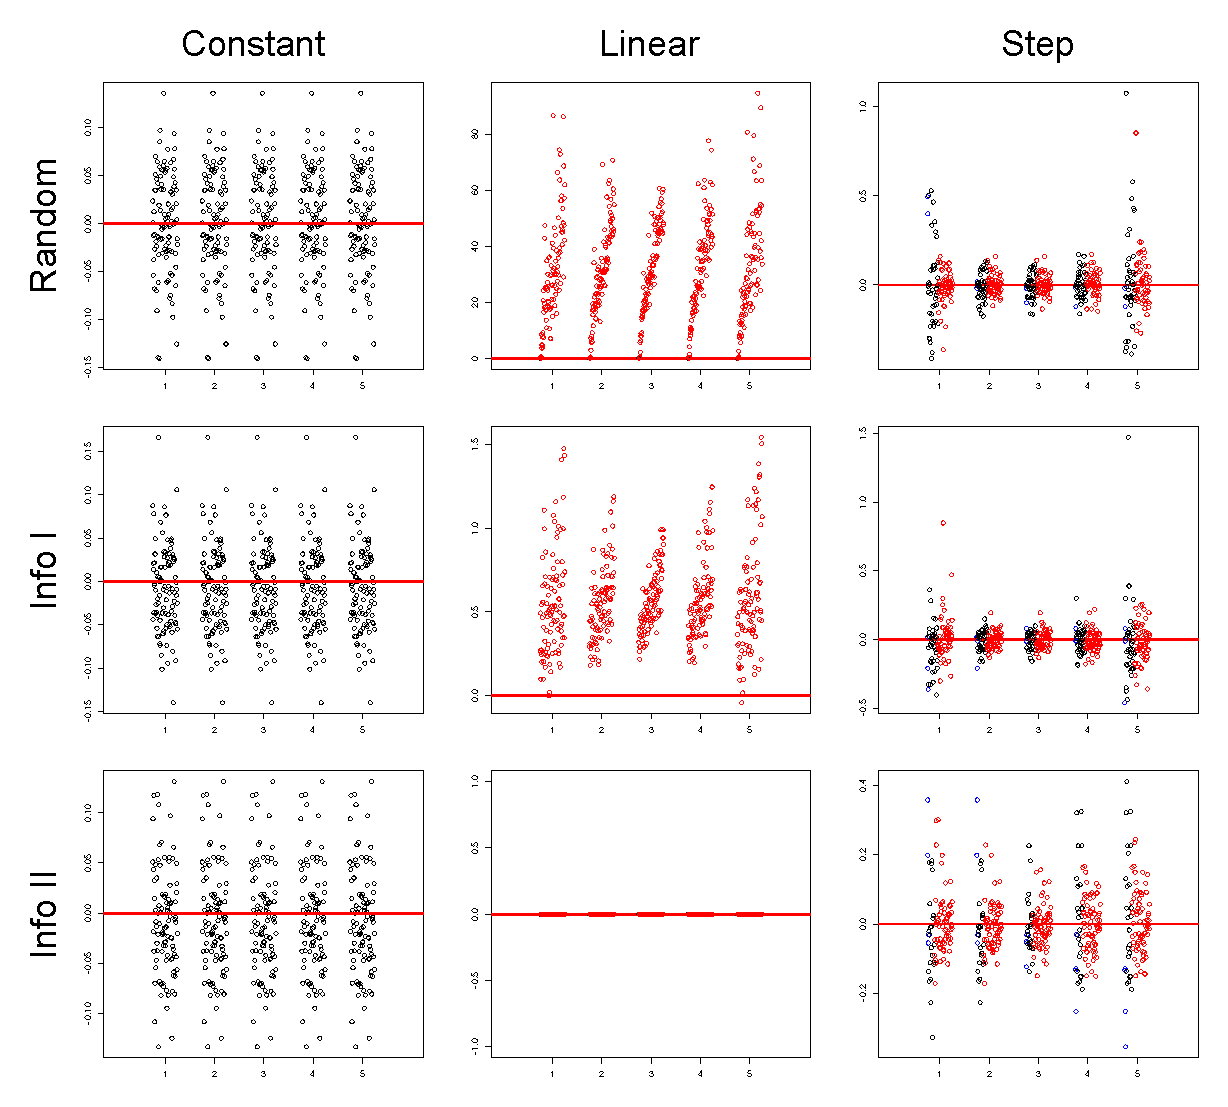
\includegraphics[scale=0.8]{Ch4_true_const_plots_2AIC_edited}
	\caption[Results from performance simulations using datasets generated with a constant evolutionary rate.]{Results from performance simulations using datasets generated with a constant evolutionary rate. Each plot shows the distance between the true value for the evolutionary rate and the estimated value for each of the 5 predictor trait categories used in the analyses. Columns show parameter estimates under different models and rows correspond to three search strategies. The x axes are the predictor trait categories from 1 to 5, y axes show $\sigma^{2}$ associated with each category. The horizontal red line marks 0, which correspond to parameter estimates equal to the true value used to generate the data. The color of the points represent AIC differences (threshold of 2 AIC units) with respect to the constant model: black points show no difference, red points are significantly worse models than the constant model, and blue points are cases in which the alternative model is better than the generating model. Each point is the mean parameter estimate across stochastic mapped histories for each of the 100 simulations. Points were slightly dislocated horizontally for better visualization.}
	\label{fig:chart_const}
\end{figure}

\begin{figure}[h]
	\centering
	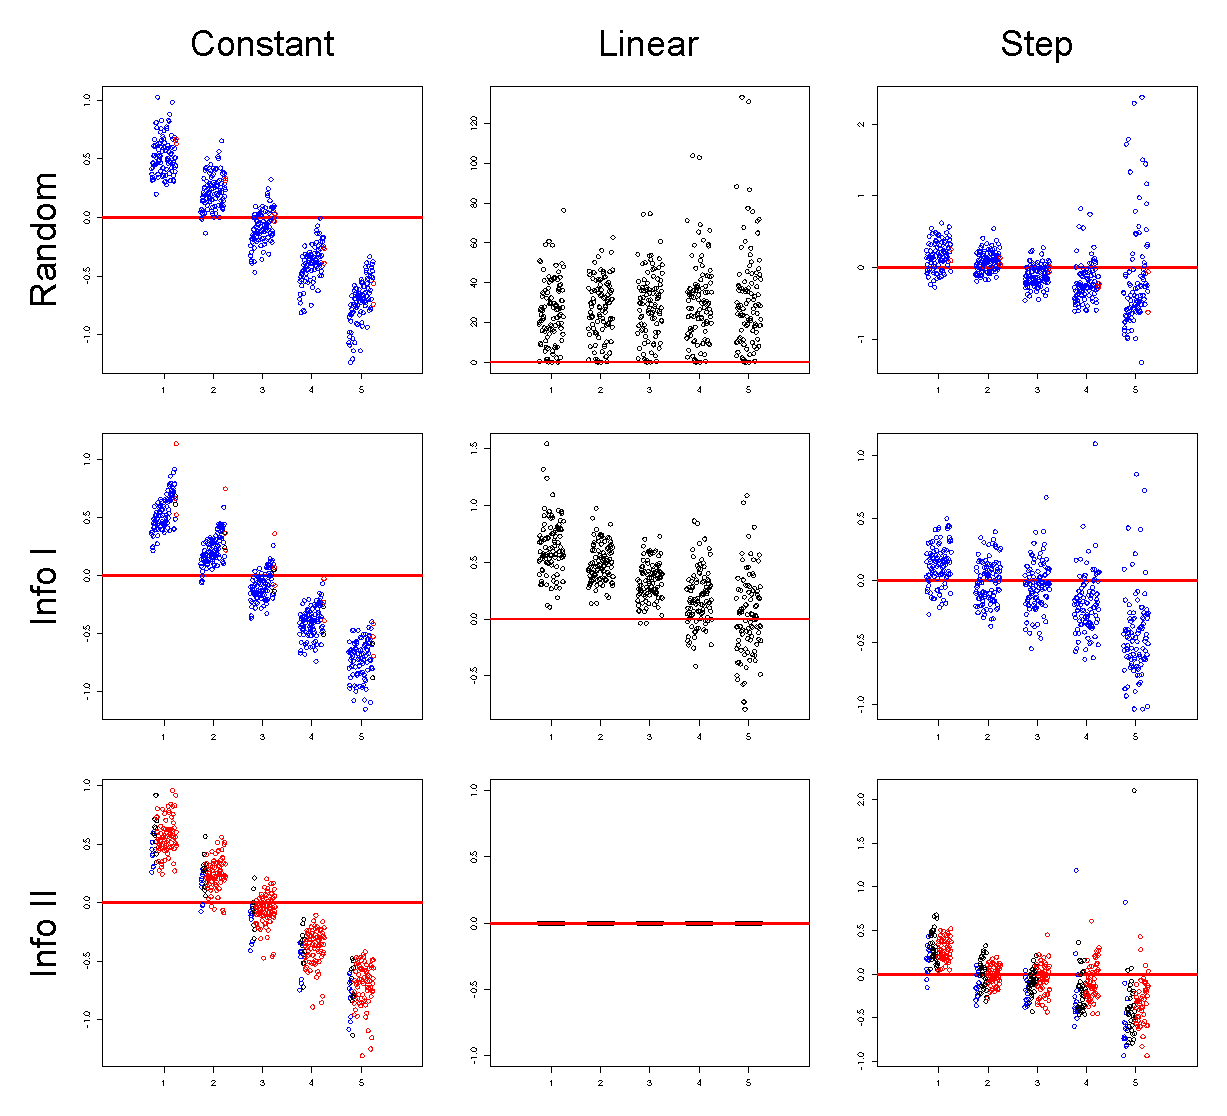
\includegraphics[scale=0.8]{Ch4_true_linear_plots_2AIC_edited}
	\caption[Results from performance simulations using datasets generated with a linear function between predictor trait values and rates of evolution of the response trait.]{Results from performance simulations using datasets generated with a linear function between predictor trait values and rates of evolution of the response trait. Each plot shows the distance between the true value for the evolutionary rate and the estimated value for each of the 5 predictor trait categories used in the analyses. Columns show parameter estimates under different models and rows correspond to three search strategies. The x axes are the predictor trait categories from 1 to 5, y axes show $\sigma^{2}$ associated with each category. The horizontal red line marks 0, which correspond to parameter estimates equal to the true value used to generate the data. The color of the points represent AIC differences (threshold of 2 AIC units) with respect to the linear model: black points show no difference, red points are significantly worse models than the linear model, and blue points are cases in which the alternative model is better than the generating model. Each point is the mean parameter estimate across stochastic mapped histories for each of the 100 simulations. Points were slightly dislocated horizontally for better visualization.}
	\label{fig:chart_linear}
\end{figure}

\begin{figure}[h]
	\centering
	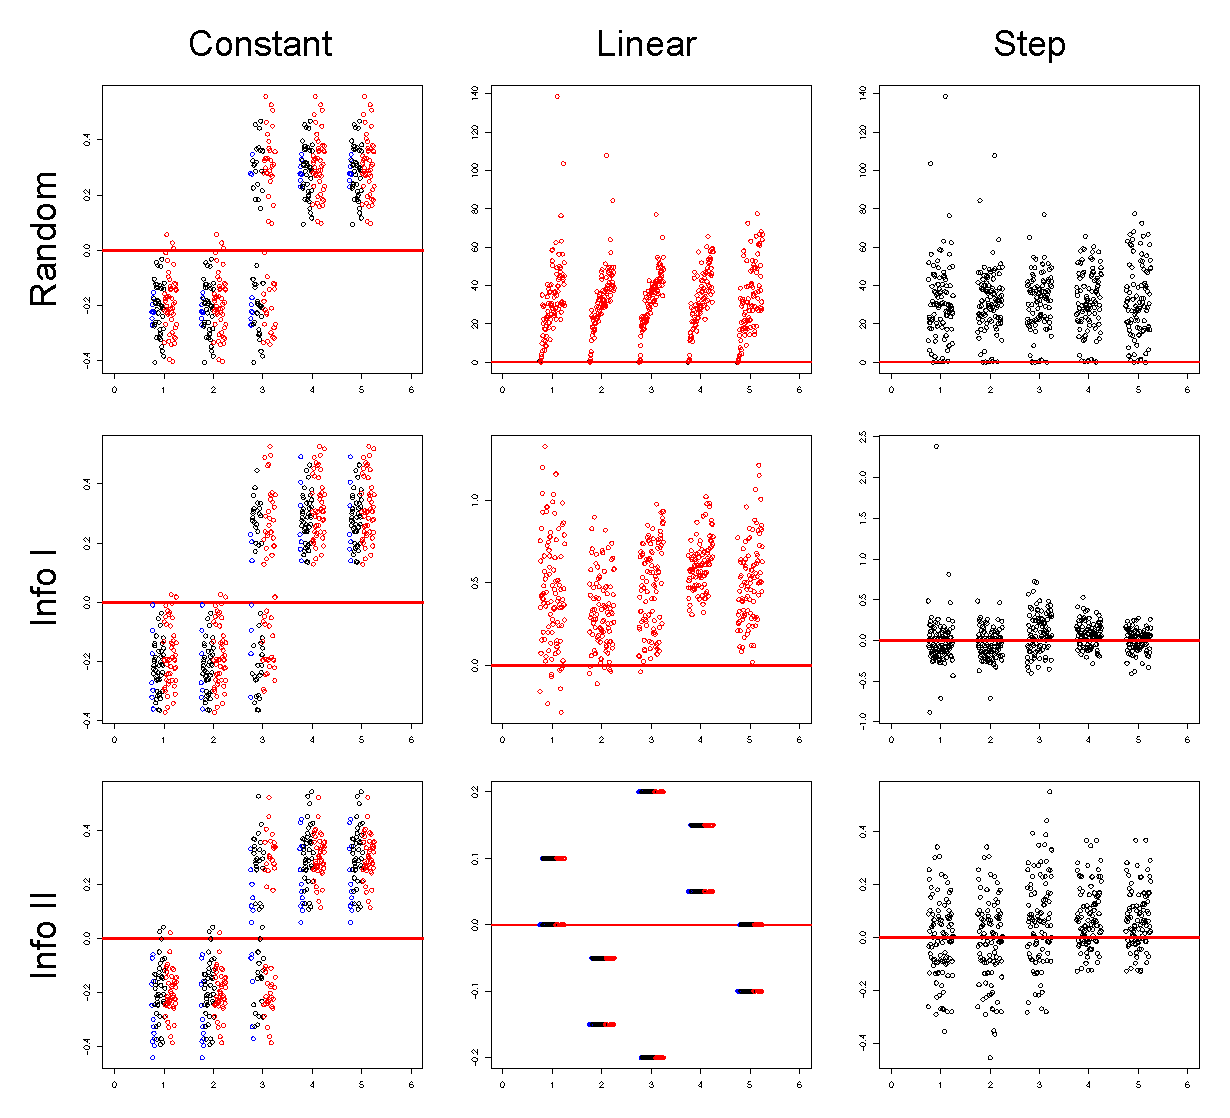
\includegraphics[scale=0.8]{Ch4_true_step_plots_2AIC_edited}
	\caption[Results from performance simulations using datasets generated with a step function between predictor trait values and rates of evolution of the response trait.]{Results from performance simulations using datasets generated with a step function between predictor trait values and rates of evolution of the response trait. Each plot shows the distance between the true value for the evolutionary rate and the estimated value for each of the 5 predictor trait categories used in the analyses. Columns show parameter estimates under different models and rows correspond to three search strategies. The x axes are the predictor trait categories from 1 to 5, y axes show $\sigma^{2}$ associated with each category. The horizontal red line marks 0, which correspond to parameter estimates equal to the true value used to generate the data. The color of the points represent AIC differences (threshold of 2 AIC units) with respect to the step model: black points show no difference, red points are significantly worse models than the step model, and blue points are cases in which the alternative model is better than the generating model. Each point is the mean parameter estimate across stochastic mapped histories for each of the 100 simulations. Points were slightly dislocated horizontally for better visualization.}
	\label{fig:chart_step}
\end{figure}